\chapter{行人导航系统实现}

\section{编码与实现}

\subsection{环境模块实现}

底层的系统环境包含一个\texttt{EnhancedPedestrianEnv}类,它是系统和虚拟仿真平台交互的底座。实现系统与虚拟仿真平台的稳定连接CarIa、地图的加载、模拟行人对象的生成与销毁、路径上起终点的设置、路径上的规划与可视化、路径上搜索时的反馈信息以及智能体对环境的感知;通过合理编码状态空间、运行控制动作、为后续算法学习和策略推理提供支持。

\subsection{奖励函数实现}

为了能够使智能体顺利地在复杂环境中完成导航任务以及避开障碍物,设计了一系列的奖励项,由于是目标导向,当智能体到达终点就给予+1000的奖励,同时为了使智能体在到达终点之前不能偏离轨迹,设计了一个在智能体偏离轨迹时就会给-500的奖励项,这个奖励项可以约束智能体沿着预设的轨迹前进,此外,在智能体与障碍物发生碰撞后给予-500的重奖,可以减少危险动作;对于智能体的避障动作以及智能体移动的速度给予奖励,使智能体在完成避障的同时以较快的速度前进,确保智能体的导航效率。

\subsection{PPO模型集成}

本系统采用\texttt{Stable-Baselines3}库中实现的 PPO算法作为主要控制策略模型。该算法在高维状态空间中表现出良好的稳定性和适应性,适用于本项目中的行人控制任务。完成状态空间与动作空间的定义后,系统对算法进行封装并结合\texttt{DummyVecEnv}接口进行训练,使模型能够连续接收来自环境的状态输入并输出相应动作决策。训练完成后,模型保存为\texttt{.zip}文件格式,以便后续部署与调用。

\subsection{GUI实现}

系统界面基于 PyQt6 开发,提供图形化操作平台,详情的用户界面截图可见附录。界面支持模型训练的控制与管理,实时显示路径导航信息,支持模型文件的导入操作,并可直接启动仿真过程。同时,日志信息以可视化方式输出,方便开发者监控系统运行状态并进行调试,提升整体使用体验。

\section{系统测试}

\subsection{测试方法}

为确保系统完整性可靠性进行测试工作采用模块单元测试与集成系统测试结合的方式。路径生成模块测试首先测试在起点终点不同组合下均能规划出一条路径,以验证路径算法的跨场景适用性,如图 \ref{fig:progress_bar}所示即在路径点范围内可用路径。

\begin{figure}[H]
    \centering
    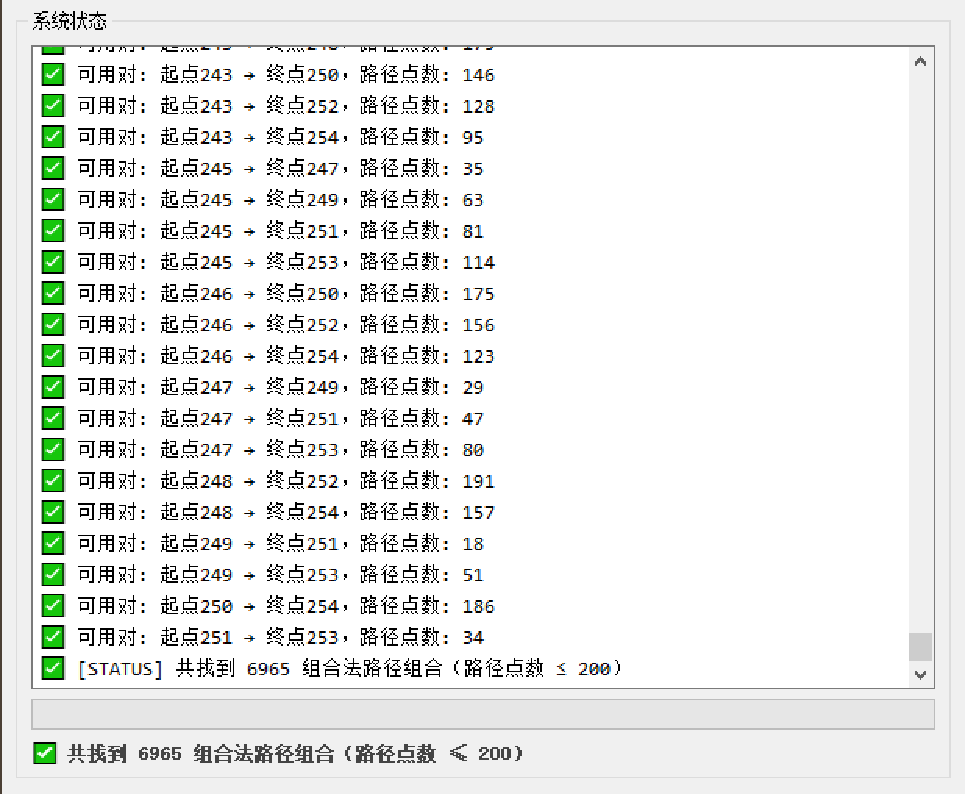
\includegraphics[width=1\textwidth]{images/available_path.pdf}
    \caption{可用路径}
    \label{fig:available_path}
\end{figure}

其次,对传感器测试感知,分别测试激光雷达和碰撞检测模块,通过不同障碍物触发条件测试激光雷达和碰撞检测模块是否及时响应和记录事件,测试传感器的数据逻辑是否处理正确。再次,奖励系统,通过不同的典型情况测试实际输出的奖励值是否和设计一致,如达到目标、偏离路径、发生碰撞、避障成功,判断奖励的激励是否合理。最后,界面交互,测试用户的操作是否被正确操作执行,各个交互按键是否正常执行,导航的路径是否正常显示在界面上,日志和状态的输出是否正常显示在界面上,测试图形界面是否完整,交互可用,通过如图 \ref{fig:progress_bar}所示的进度条管理来反馈此时的训练进程给用户。

\begin{figure}[H]
    \centering
    \includegraphics[width=1\textwidth]{images/progress_bar.pdf}
    \caption{运行进度条}
    \label{fig:progress_bar}
\end{figure}

\subsection{测试结果}

系统经不同路径,场景的测试,在路径规划、障碍检测、UI交互、奖励回馈等关键方面都具备较强的稳定性、高效性。表 \ref{tab:test-results} 汇总了主要测试模块的结果。

\begin{table}[H]
    \centering
    \caption{系统测试结果汇总}
    \label{tab:test-results}
    \renewcommand{\arraystretch}{1.3}
    \begin{tabular}{
        >{\centering\arraybackslash}p{4cm}
        >{\centering\arraybackslash}p{3cm}
        >{\centering\arraybackslash}p{6cm}
    }
    \toprule
    \textbf{测试模块} & \textbf{结果} & \textbf{备注} \\
    \midrule
    路径规划 & 成功 & 最长路径点数 96 个 \\
    避障检测 & 正确响应 & 成功避障率 95\% \\
    GUI 交互 & 正常 & 控件无卡顿 \\
    奖励反馈 & 正确计算 & 终止条件有效 \\
    \bottomrule
    \end{tabular}
\end{table}

路径规划实验过程中,所有起始点和目标点都不相同的情况下,都能够规划出一条路径,路径最长点数为96,表明路径规划算法适应性强,稳定性好。避障检测实验,分别设置不同种类的静态、动态障碍物,系统检测与避障均能够被触发,系统避障率为95\%,表明避障检测实验能够较好检测到障碍物,对环境的适应性强。图形界面操作实验测试,交互按键均能够被系统快速识别,系统的训练、导入、模拟等操作没有出现卡帧、延时情况,图形界面显示的按键都能正常使用,系统交互操作较为稳定。奖励反馈方面,系统在满足结束条件(到达、碰撞)时均能够及时显示出相应的结果与惩罚,系统奖励与惩罚功能逻辑清晰准确,且稳定工作,对智能体的学习具有较好的指导意义。

\section{系统数据管理}

行人在进行导航系统的训练与测试中,会涉及到大量与行走、路径规划、避障、强化学习相关的数据,为了便于保存,便于统一管理,便于后期分析,设计了轻量级数据库。

本节介绍数据库架构、数据来源、表结构设计、记录逻辑以及数据库在模型训练与评估中的应用。

\subsection{地图与可行走区域设置}

导航系统使用CARLA平台中的Town01地图作为基础环境,地图结构包含道路、建筑、人行道与交通标志等元素。为构建有效导航起点与终点,系统预先提取可行走区域点集,并将其以CSV格式保存为walkable\_points\_Town01.csv。该文件记录了地图中经过筛选的可通行坐标点,字段包含x、y、z三维坐标,其中z值统一为0.3表示地面层高度,如下表所示。

\begin{table}[H]
    \centering
    \caption{部分可通行坐标点数据表}
    \label{tab:coord_data}
    \begin{tabular}{cccc}
        \toprule
        index & $x$ & $y$ & $z$ \\
        \midrule
        0 & 335.4899 & 273.7433 & 0.3000 \\
        5 & 272.2900 & 59.3301 & 0.3000 \\
        6 & 272.2900 & 55.8400 & 0.3000 \\
        9 & 202.5500 & 59.3301 & 0.3000 \\
        10 & 202.5500 & 55.8400 & 0.3000 \\
        11 & 92.1100 & 227.2200 & 0.3000 \\
        13 & 191.0800 & 55.8400 & 0.3000 \\
        17 & 158.0800 & 27.1800 & 0.3000 \\
        18 & 295.0818 & 199.0603 & 0.3000 \\
        19 & 295.0818 & 195.5703 & 0.3000 \\
        \bottomrule
    \end{tabular}
\end{table}

地图的原始格式存储为.pcd和.bin文件,分别表示点云文件和生成地图路径图文件,在路径生成和障碍物探测方面进行。根据实际情况,有些区域障碍物比较多,系统就跳过障碍物,路径生成以目标点在无障碍的区域内为原则。

\subsection{模型与数据融合}

系统采用PPO强化学习算法进行路径控制训练,训练过程中使用EnhancedPedestrianEnv作为交互环境,执行策略动作后将轨迹反馈、奖励变化与环境观测存储至数据库。模型训练模块封装于TrainingWrapper类,周期性保存模型参数至.zip格式,并记录每轮训练的统计指标。

系统训练流程中由trajectory\_log写入路径轨迹,collision\_events记录碰撞反馈,training\_summary跟踪整体表现。模型文件最终保存为pedestrian\_ppo.zip,包含策略网络权重与环境配置,便于复现与迁移。图\ref{fig:progress_bar}即为保存下来的模型压缩包内部文件。

\begin{figure}[H]
    \centering
    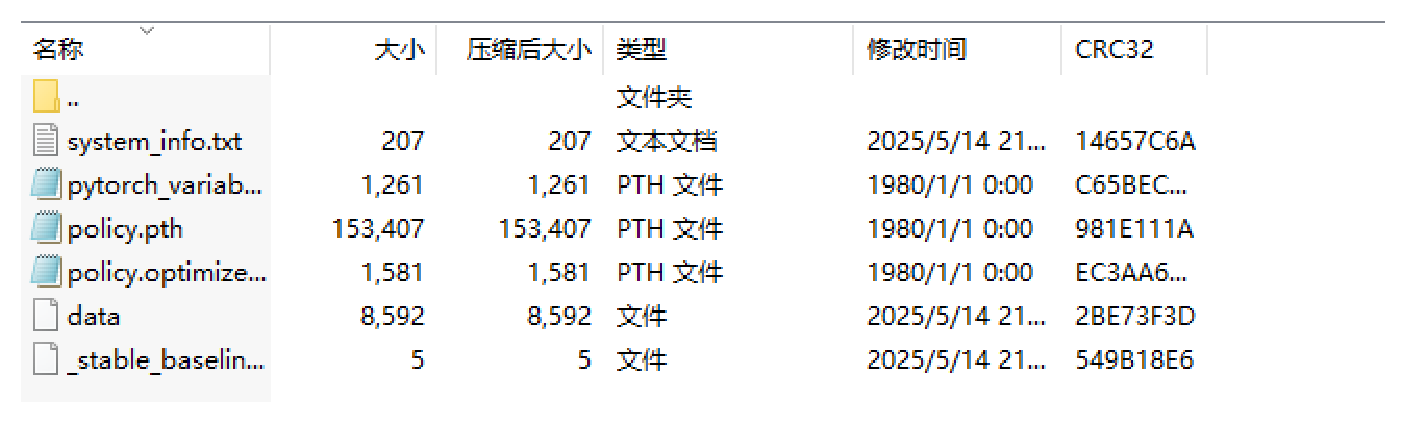
\includegraphics[width=1\textwidth]{images/model.pdf}
    \caption{模型文件}
    \label{fig:model}
\end{figure}

GUI系统提供演示功能,加载模型并自动运行路径导航,期间继续采集数据并补充至数据库,支持实验复验与可视化重构。

该流程构建数据生成、模型训练与效果评估闭环,数据库不仅承担记录任务还作为策略分析与系统评估的基础核心。

\section{系统部署与维护}

\subsection{部署方案}

本文系统支持本地部署,硬件环境推荐 CPU 为英特尔 i7、硬盘 16G 及以上,部署前需预先安装 Carla 仿真平台及 PyQt6、stable-baselines3、gymnasium 等 Python 依赖库以确保系统正常运行,整个部署流程简洁,用户可按附录用户手册操作,主要步骤如下:

\begin{enumerate}
    \item 启动 Carla 仿真服务以初始化虚拟环境;
    \item 运行系统图形界面程序,进入主控制面板;
    \item 在界面中选择起始点与目标点,用户可选择重新训练强化学习模型,或加载已有模型直接进入导航仿真流程。
\end{enumerate}

上述部署过程可在具备基础开发经验的条件下快速完成,模块化架构设计也为系统的跨平台适配与扩展提供了便利。

\subsection{后期维护与优化}

系统发生的所有重要的事件、状态的日志被记录在日志系统中,并且在图形化界面的状态栏中显示,如图 \ref{fig:gui-log} 所示。日志显示系统正在进行什么操作,或者检测到错误正在报警。当系统检测到错误或者报警时,在系统中会出现位置和类型,开发人员可以依据位置在源代码中定位修复错误。

\begin{figure}[H]
    \centering
    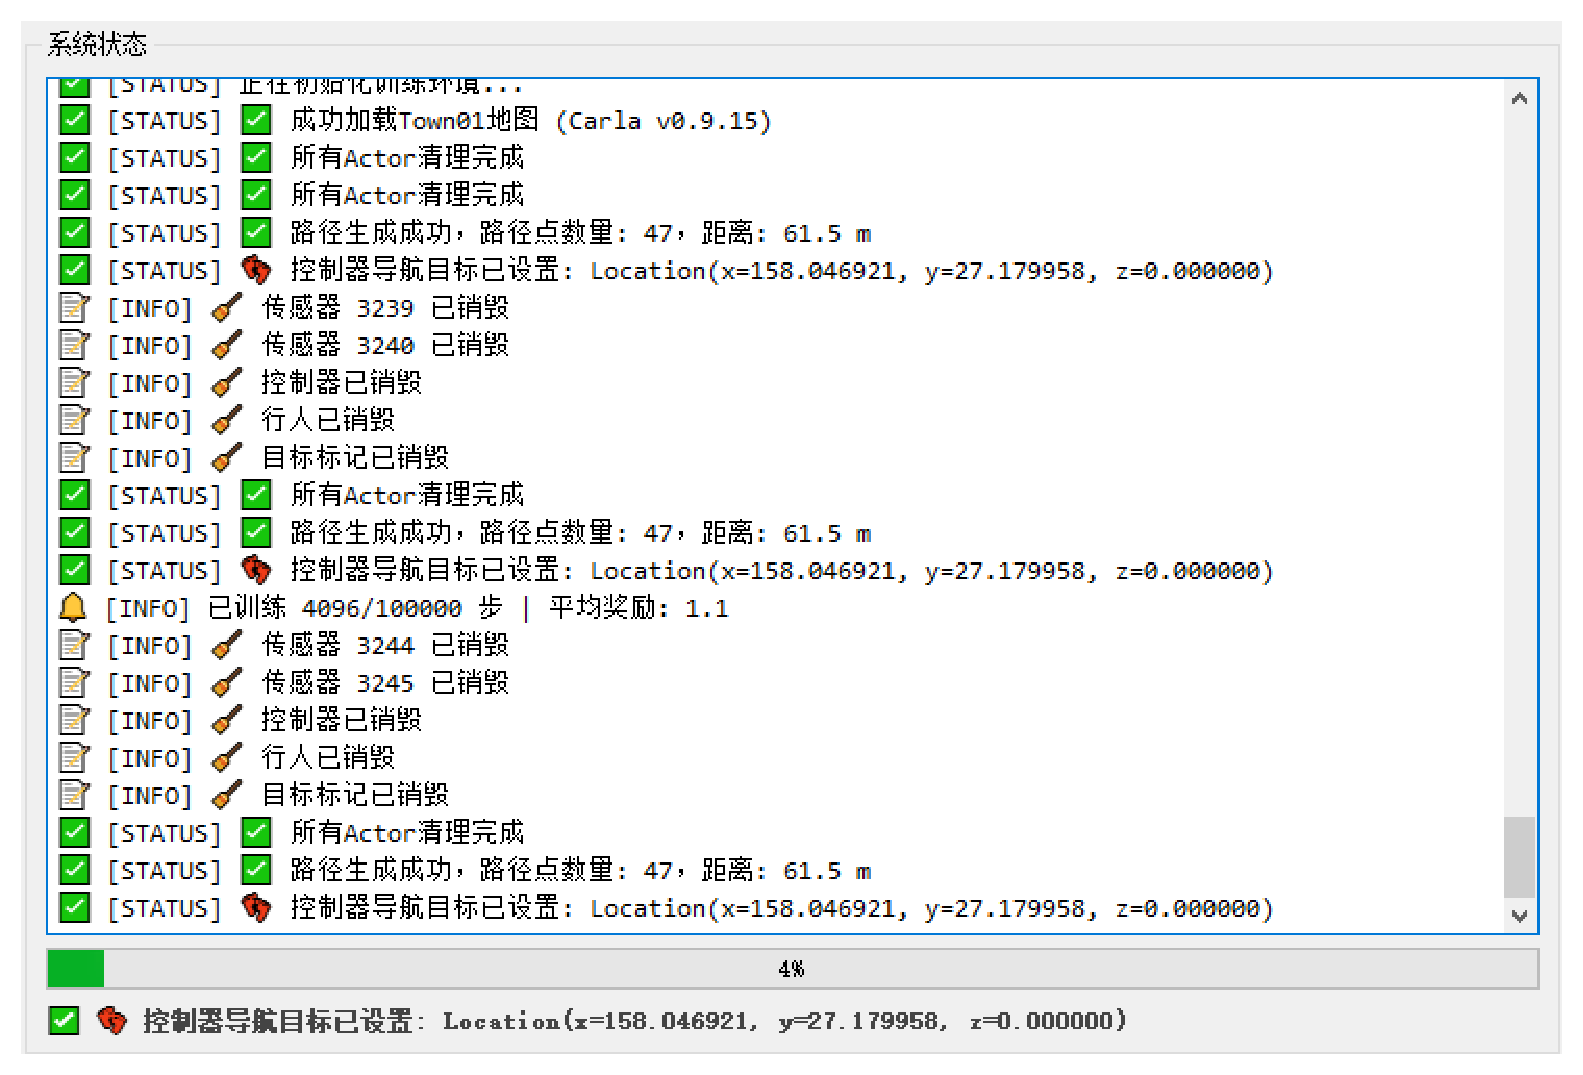
\includegraphics[width=1\textwidth]{images/gui_log.pdf}
    \caption{日志显示截图}
    \label{fig:gui-log}
\end{figure}

为了提高系统可维护性,源程序的结构采用模块式的结构,对系统进行数据处理、策略学习、图形界面、仿真交互的划分,降低了它们之间的耦合性,让用户在维护的过程中便于对系统进行修改,并且便于使用者对系统进行个性化修改。

在完善方面,系统是可拓展的,后续可以设计多智能体协作,在更密集的交通环境中展开行人合作博弈实验;系统可以加载更复杂的仿真地图(Town02、Town03、Town04、Town05、Gender5),进一步测试模型在高密度交通环境中的泛化能力。同时,通过结合目标检测(如YOLO系列),动态识别对象、设计行为预测模块实现前瞻性规避障碍策略,能进一步提升系统应对动态变化的鲁棒性与智能性。

\section{本章小结}

本章主要对行人导航系统的具体搭建进行详细说明,在虚幻引擎和Carla的基础上,对系统的环境生成、模型部署、界面设计、数据管理等进行了实现。首先对系统的代码流程以及具体模块进行介绍,完成了PPO模型的部署以及多维奖励函数,然后设计了键盘和GUI操作进行用户体验,最后完成了仿真环境内行人导航过程的显示。最后对路径长短、避障情况和路径正确与否等指标进行了测试和分析,在系统具体实现方面,本文对系统复杂环境的适应性以及可靠性进行了证明,对日后的研究工作有很大的借鉴意义。本章完成了系统的初步实现,为之后系统分析工作做出了铺垫。本系统的初步实现说明系统具备一定的完整性和可开发性,之后可以进行系统分析和系统改进工作。
